\documentclass[a4paper,twocolumn,8pt]{extarticle}

\usepackage{pscyr}
\usepackage[utf8]{inputenc}
\usepackage[english, russian]{babel}

\usepackage{extsizes}
\usepackage[a4paper,top=0.5cm,bottom=1.0cm,left=1.0cm,right=0.5cm,nomarginpar,foot=0.3cm,includehead]{geometry}
\usepackage{lastpage}
\usepackage{listings}
\usepackage{xcolor}
\usepackage{fancyhdr}
\usepackage{amssymb}
\usepackage{hyperref}
\usepackage{graphicx}

\hypersetup{
    colorlinks=true,
    linkcolor=black,
    filecolor=magenta,
    urlcolor=blue,
}

\definecolor{codegreen}{rgb}{0,0.6,0}
\definecolor{codegray}{rgb}{0.5,0.5,0.5}
\definecolor{codepurple}{rgb}{0.58,0,0.82}
\definecolor{backcolour}{rgb}{1,1,1}

\lstdefinestyle{codestyle}{
    language=C++,
    backgroundcolor=\color{backcolour},
    commentstyle=\color{codegreen},
    keywordstyle=\color{magenta},
    stringstyle=\color{codepurple},
    basicstyle=\ttfamily,
    breakatwhitespace=false,
    breaklines=true,
    captionpos=b,
    keepspaces=true,
    numbersep=5pt,
    showspaces=false,
    showstringspaces=false,
    showtabs=false,
    tabsize=2
}

\lstset{
    style=codestyle,
    extendedchars=\true,
%    literate=
%        {б}{{\selectfont\char225}}1
%        {в}{{\selectfont\char226}}1
%        {г}{{\selectfont\char227}}1
}
\setlength{\columnseprule}{0.4pt}
\setlength{\columnsep}{30pt}

\begin{document}
    \pagestyle{fancy}
    \fancyhead[LO]{St. Petersburg State University (Ushakov, Turevskii, Danilevich)}
    \fancyhead[R]{Page \thepage~of~\pageref{LastPage}}
    \tableofcontents
    \newpage
    \section{Настройка CLion}
\begin{enumerate}
    \item В файле \texttt{CMakeLists.txt} дописать строчку \texttt{add\_compile\_definitions(LOCAL)}.
    Нажать появившуюся опцию в правом верхнем углу \texttt{enable auto-reload}.
    \item Вбить шаблон в \texttt{main.cpp}:
    \lstinputlisting{template.cpp}
    Скомпилировать, чтобы проверить отсутствие опечаток.
    \item Запустить терминал (crtl + alt + T)
    \begin{lstlisting}
$ cd workspace/CLionProjects
$ for c in {A..Z}; do cp main.cpp $c.cpp && echo "add_executable($c $c.cpp)" >> CMakeLists.txt; done\end{lstlisting}
\end{enumerate}
Далее отключаем подсветку и форматирование в настройках (ctrl+alt+S)
\begin{itemize}
    \item Editor $\to$ Inlay Hints $\to$ отключаем всё (достаточно первых трёх --- code vision, parameter names, types).
    \item Editor $\to$ Code Style $\to$ Formatter $\to$ \texttt{Do not format} прописать \texttt{*}
    \item Editor $\to$ Inspections $\to$ C/C++ $\to$ static analysis tools $\to$ CLang-Tidy отключить
\end{itemize}
    \section{Теория чисел}
    \subsection{КТО}
\lstinputlisting{algos/chinese remainder theorem/chinese remainder theorem.cpp}
% https://codeforces.com/contest/982/submission/230056019

    \subsection{Алгоритм Миллера --- Рабина}
\lstinputlisting{algos/miller rabin/miller rabin.cpp}
    \subsection{Алгоритм Берлекэмпа --- Месси}
\underline{\url{https://mzhang2021.github.io/cp-blog/berlekamp-massey/}}
\lstinputlisting{algos/berlekamp massey/berlekamp massey.cpp}

    \section{Графы}
    \subsection{$\mathcal{SCC}$ и 2-$\mathcal{SAT}$}
Алгоритм ищет сильносвязные компоненты в графе $g$, если есть путь $i \rightarrow j$, то $scc[i] \le scc[j]$

\lstinputlisting{algos/SCC and 2SAT/SCC.cpp}
Чтобы решать 2-$\mathcal{SAT}$, надо создать граф на $2n$ вершинах, рёбра $i \Rightarrow j$ и $(j\oplus1) \Rightarrow (i \oplus 1)$ должны быть добавлены одновременно.
После этого если \texttt{scc[2 * i] = scc[2 * i + 1]}, то решения нет; если \texttt{scc[2 * i + 0] < scc[2 * i + 1]}, то присутствует импликация $\neg i \Rightarrow i$, надо назначить $i = $\texttt{true}.

%https://codeforces.com/contest/228/submission/230077013
%https://judge.yosupo.jp/submission/168750
%https://judge.yosupo.jp/submission/168753

    \subsection{Эйлеров цикл}
\lstinputlisting{algos/euler/euler.cpp}
% https://codeforces.com/gym/102935/submission/230083828
    \subsection{Компоненты рёберной двусвязности}
\lstinputlisting{algos/edge-2-connectivity/edge-2-connectivity.cpp}
% https://qoj.ac/submission/281898
    \subsection{DCP offline}
\lstinputlisting{algos/dcp offline/dcp-offline.cpp}
    \subsection{Взвешенное паросочетание}
\underline{\url{https://judge.yosupo.jp/submission/201334}}
\lstinputlisting{algos/general weighted matching/1.cpp}
\lstinputlisting{algos/general weighted matching/2.cpp}
\lstinputlisting{algos/general weighted matching/3.cpp}


    \section{Cвёртки}
    \subsection{XOR свёртка}
%\lstinputlisting{algos/bit convolutions/band.cpp}
%\lstinputlisting{algos/bit convolutions/bor.cpp}
\lstinputlisting{algos/bit convolutions/bxor.cpp}
    \subsection{FFT \& co}
\lstinputlisting{algos/fft/fft-998244353.cpp}
\subsection{Быстрое FFT}
\begin{itemize}
    \item Solution based on \underline{\url{https://codeforces.com/blog/entry/117947}}
    \item Iterative and in-place version.
    \item Uses signed montgomery
    \item Optimized to minimize memory usage
\end{itemize}
\lstinputlisting{algos/fft/fast-fft-998244353.cpp}
\subsection{FFT в double'ах}
\lstinputlisting{algos/fft/fft-double.cpp}


    \section{Структуры данных}
    \subsection{Дерево Фенвика}
\lstinputlisting{algos/segment tree and fenwick/fenwick.cpp}
\subsection{Дерево отрезков в точке}
\lstinputlisting{algos/segment tree and fenwick/point-segment-tree.cpp}
\subsection{Массовое дерево отрезков}
\lstinputlisting{algos/segment tree and fenwick/mass-segment-tree.cpp}

    \subsection{Битовый бор}
\lstinputlisting{algos/bit trie/bit trie.cpp}
    \subsection{Ordered set}
\lstinputlisting{algos/ordered set/ordered set.cpp}
    \subsection{Convex hull trick}
\lstinputlisting{algos/cht/cht.cpp}
    \subsection{Центроиды}
\lstinputlisting{algos/centroids/centroids.cpp}
    \subsection{Дерево Ли Чао}
\lstinputlisting{algos/li-chao/li-chao.cpp}

    \subsection{Min-Kinetic Segment Tree}
I guess the source is https://koosaga.com/307
\lstinputlisting{algos/min-kinetic-segment-tree/kst.cpp}

    \section{Строковые алгоритмы}
    \subsection{Префикс-функция}
\lstinputlisting{algos/prefix-function/prefix-function.cpp}
    \subsection{$Z$-функция}
\lstinputlisting{algos/z-function/z-function.cpp}
    \subsection{Алгоритм Манакера}
\lstinputlisting{algos/manacher/manacher.cpp}
    \subsection{Суфмассив}
Переработанный китайский суффмассив
\lstinputlisting{algos/sufarray/sa.cpp}

    \subsection{Алгоритм Ахо --- Корасик}
    \lstinputlisting{algos/aho corasick/aho-corasick.cpp}

    \subsection{Дерево палиндромов}
    \subsection{Дерево палиндромов}
\lstinputlisting{algos/palindromic tree/palindromic tree.cpp}

    \section{Потоки}
    \subsection{Алгоритм Диница}
\lstinputlisting{algos/dinic/dinic.cpp}
    \subsection{Mincost k-flow}
\lstinputlisting{algos/mincost k-flow/mincost k-flow.cpp}
\lstinputlisting{algos/mincost k-flow/mincost maxflow.cpp}


    \section{Гамильтоновы путь и цикл}
\underline{\url{https://codeforces.com/blog/entry/90513}},
\underline{\url{https://codeforces.com/blog/entry/90743}}.
\subsection{Link-cut tree}
\lstinputlisting{algos/hamiltonian/LCT.cpp}
\subsection{Undirected case}
\lstinputlisting{algos/hamiltonian/undirected.cpp}
\subsection{Directed case}
\lstinputlisting{algos/hamiltonian/directed.cpp}

    \section{Геома}
    \subsection{Примитивы}
\lstinputlisting{algos/geometry/geomPrim.cpp}
\subsection{Выпуклая оболочка}
\lstinputlisting{algos/geometry/convex hull.cpp}
\subsection{Точка внутри многоугольника}
\lstinputlisting{algos/geometry/inPolygon.cpp}
\subsection{Касательные}
\lstinputlisting{algos/geometry/tangents.cpp}
\subsection{Пересечение многоугольника и полуплоскости}
\lstinputlisting{algos/geometry/intersection.cpp}
\subsection{События для прямой}
\lstinputlisting{algos/geometry/events.cpp}
    \section{Цепные дроби}
\underline{\url{https://cp-algorithms.com/algebra/continued-fractions.html}}
\subsection{Поиск нижней огибающей, сумма и минимум по модулю}
\lstinputlisting{algos/continued fractions/cf.cpp}
\subsection{Простая рекурсия}
Число точек $(x, y) : 0 \leqslant x < n, 0 < y \leqslant (kx + b) / d$.
То есть $\sum\limits_{x=0}^{n-1} \lfloor\frac{kx+b}{d}\rfloor$.
\lstinputlisting{algos/continued fractions/recursion.cpp}
    \section{Разное}
    \subsection{Нимы}
По умолчанию проигрывает тот, кто не может сделать ход.
\begin{enumerate}
\item Полоска $1\times n$. Надо ставить крестик в незанятую клетку, нельзя ставить в соседние.
\textbf{Решение:} динамика за $\mathcal{O}(n^2)$. Оказывается, начиная с $n = 52$ есть период длины $34$.
\item Полоска $1\times n$. Надо ставить крестик в незанятую клетку. Выигрывает тот, кто получит три крестика подряд. \textbf{Решение:} как в (1), только крестик банит слева и справа по две клетки.
\item Доска $3 \times n$, изначально стоят $n$ белых пешек в первом ряду, $n$ чёрных в последнем. Правила шахматные, но бить обязательно. \textbf{Решение: } совпадает с (1).
\item Ним, но ещё за ход разрешается вместо взятия камней разделить какую-то кучку на две. \textbf{Решение:} динамика за квадрат. Оказывается, $g[n] = n + s_n$, где $s_n = 1$ для $n \equiv 3 \pmod{4}$, $s_n = -1$ для $n \equiv 0 \pmod {4}$, $s_n = 0$ в остальных случаях (и, конечно, при $n = 0$).
\item Полоска $1 \times n$. Надо поставить крестик в незанятую клетку, или пару крестиков в соседние незанятые клетки. \textbf{Решение:} динамика за квадрат. Оказывается, начиная с некоторого места $(n = 60?)$ последовательность периодична с периодом $12$.
\item $n$ кучек камней. Надо разделить кучку размера $\ge 3$ на две неравные. \textbf{Решение:} динамика за квадрат. Период неизвестен человечеству.
\item $n$ кучек камней. Надо переместить ненулевое число камней из $i$-й кучки в $(i-1)$-ю (для $i > 1$). \textbf{Решение:} нимбер --- это $a_2 \oplus a_4 \oplus a_6 \oplus \dots$, так как это ним с увеличениями.
\item Полоска $1 \times n$, на ней $k$ фишек. Надо переместить любую фишку куда-то влево, не перепрыгивая и не вставая на другие фишки. \textbf{Решение:} сводимся к предыдущей задаче
\item Полоска $1 \times n$, в каждой клетке $o$ илм $x$. Надо поменять $o$ на $x$, после чего (разрешается|надо) флипнуть знак где-то слева. \textbf{Решение:} нимбер --- $\oplus$-сумма координат нулей (в $1$|в $0$)-индексации.
\item Полоска $1 \times n$, в ней стоят две фишки $I$ и $I\:I$. Игрок берёт свою фишку, и перемещает на ненулевое число клеток, не перепрыгивая и не вставая на фишку противника. \textbf{Решение:} нимбер --- число клеток между фишками.
\item Доска $2 \times n$. Надо поставить крестики в $3$ незанятые клетки вида триомино (связная по сторонам фигура из трёх клеток, не лежащих на одной прямой). \textbf{Решение:} динамика за квадрат --- фигуру площади $n$ всегда можно разбить на $k$ и $n-3-k$.
\item Ним-Баше: можно брать не более $k$ предметов. \textbf{Решение: } эквивалентно ниму с состояниями $a_i \pmod{(k+1)}$.
\item Ним Мура: можно брать сколько угодно из не более, чем $k$ кучек. \textbf{Решение:} проигрышная тогда и только тогда если взять все кучки, записанные в двоичной системе счисления, то в каждом бите сумма делится на $(k+1)$.
\item Ним в поддавки: \textbf{Решение:} нимбер --- $a_1 \oplus \ldots \oplus a_n \oplus [\text{все }a_i \le 1]$.
\end{enumerate}
\subsection{Компараторы}
\lstinputlisting{algos/comparators guide.cpp}
\subsection{Трюки от Сергея Копелиовича}
\subsubsection{Быстрый ввод}
\underline{\url{https://acm.math.spbu.ru/~sk1/algo/input-output}}
\lstinputlisting{algos/fast-input.cpp}
\lstinputlisting{algos/read_double.cpp}
\underline{\url{https://acm.math.spbu.ru/~sk1/algo/memory.cpp.html}}
\subsubsection{Быстрый аллокатор}
\lstinputlisting{algos/bump-alloc.cpp}
\subsection{Редукция Барретта}
\lstinputlisting{algos/barrett.cpp}
\subsection{Флаги компияции}
\texttt{-DLOCAL -Wall -Wextra -pedantic -Wshadow -Wformat=2 -Wfloat-equal -Wconversion -Wlogical-op -Wshift-overflow=2 -Wduplicated-cond -Wcast-qual -Wcast-align -D\_GLIBCXX\_DEBUG -D\_GLIBCXX\_DEBUG\_PEDANTIC -D\_FORTIFY\_SOURCE=2 -fsanitize=address -fsanitize=undefined -fno-sanitize-recover -fstack-protector -std=c++2a}
%\subsubsection{Сеточка в vim}
%\underline{\url{https://codeforces.com/blog/entry/122540}}
%\begin{lstlisting}
%i|<esc>25A   |<esc>
%o+<esc>25A---+<esc>
%Vky35Pdd
%\end{lstlisting}
\subsection{Что сделать на пробном туре}
\begin{itemize}
\item Послать клар
\item Распечатать что-то
\item Получить ML (stack \& heap)
\item Максимальный размер отправляемого файла?
\item Убедиться, что чекер регистронезависимый (yes/YES)
\item Позапускать Флойда --- Варшалла
\item Посмотреть, насколько быстр быстрый ввод
\item Перебить что-то, проверить хеш
\item Проверить санитайзеры
\end{itemize}
\subsection{Хеш файла без комментариев}
Хеш файла, игнорирующий переводы строк и комментарии:
\begin{lstlisting}
$ cpp -dD -P -fpreprocessed "$filename" | tr -d '[:space:]' | md5sum | cut -c-6
\end{lstlisting}
\begin{verbatim}__builtin_ia32_ldmxcsr(40896);\end{verbatim}

%    \clearpage
%    
\includegraphics{hexagonal.ps}
%    \clearpage
%    \includegraphics{triangle.ps}
%    \clearpage
\end{document}
